\chapter{Hashing}
\label{chapter-hashing}
Hashing is one of the approaches designed for efficient solving of the dictionary problem. Various implementations differ in many different ways. However usage of a hash function and a quickly accessible table, typically represented by an array, is common to the most of them. Hash function transforms elements of the universe into addresses of the table.

Represented sets are always small when compared to the size of the universe. In order to prevent waste of space we are forced to use tables as small as possible. Typically the size of the table storing the represented elements is chosen so that it is comparable to those of the stored set. 

The fact that the hash table is much smaller than the possible universe and any two elements can be included in the represented set means that the elements may share the same address after using the hash function. This event is called a \emph{collision}. For hashing it is very important how collisions are handled. This is also the most interesting distinctive feature for different hashing models. In fact collision handling is crucial when determining the time complexity of the scheme.

When two elements collide they should be stored in a single \emph{bucket}, cell of the hash table. A bucket is often represented by the simplest data structure possible. For instance single linked list should be sufficient in many cases. In more sophisticated schemes, like perfect hashing, another hash table is used. 

For imagination the find operation of a hash table works in the following way. Every element is put as an argument of a hash function. The element's address is then computed and used as an index of the hash table. Then we look into the bucket lying at the returned address if the element is stored inside it or not.

\begin{figure}
  \centering
    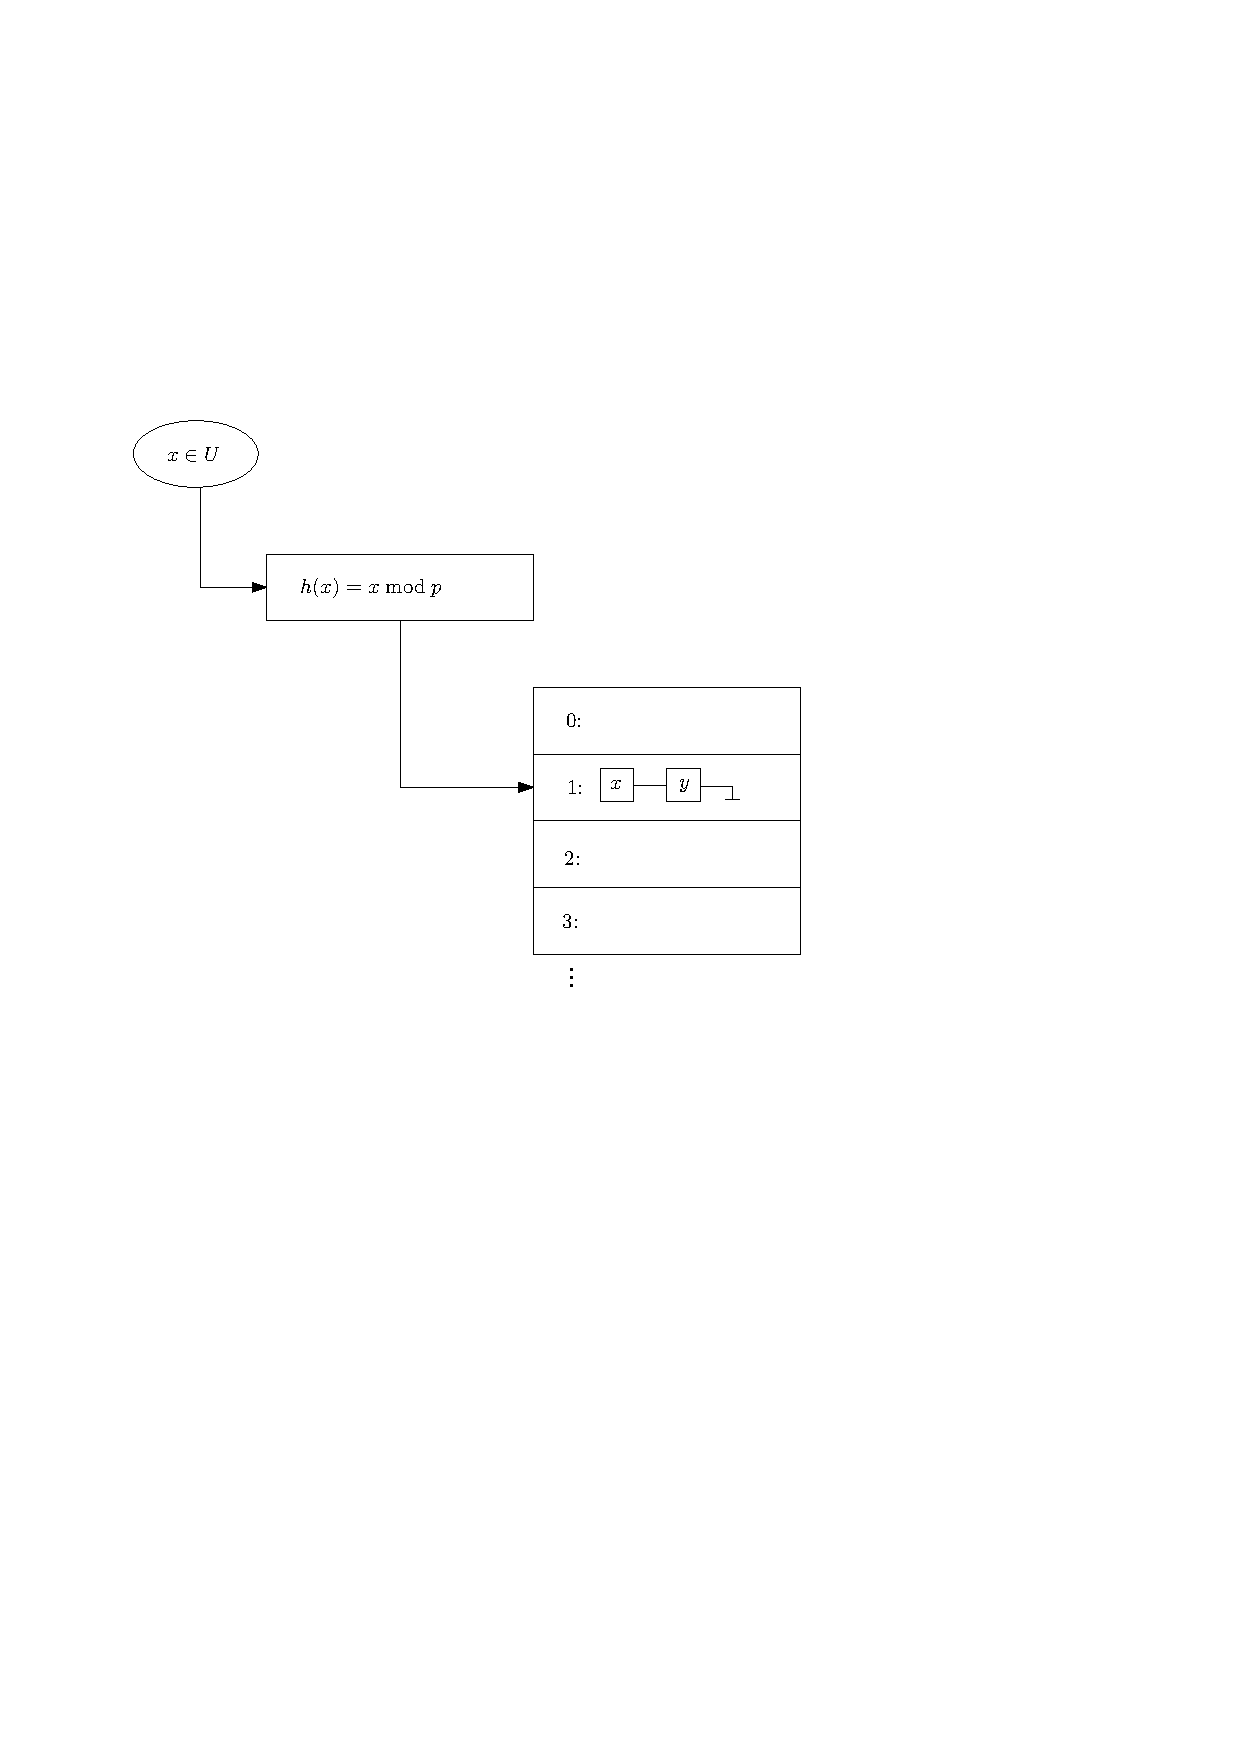
\includegraphics[width=0.5\textwidth]{images/hash_table}
  \caption{Concept of a hash table.}
\end{figure}

If we represent buckets by singly linked lists the expected time of the find operation is proportional to the half of the length of the list.
\begin{lemma}
\label{lemma-expected-list-time}
Let $S$ be a set represented by a singly linked list. Moreover assume that for every element $x \in S$: \[ \Prob{x \text{ is argument of the find operation}} = \frac{1}{|S|} \text{.} \] Then the expected time of the find operation is $\frac{|S| + 1}{2}$.
\end{lemma}
\begin{proof}
Let $x_i \in S$ be the $i$-th element of the list for $1 \leq i \leq |S|$. Time to find the element $x_i$ inside the list equals $i$. The expected time of the find operation can be expressed directly from its definition. 
\[
\begin{split}
\Expect{\text{time of the find operation}} 
	& = \displaystyle\sum_{i = 1}^{|S|} i \Prob{x_i \text{ is the argument of the find operation}} \\
	& = \frac{\sum_{i = 1}^{|S|}{i}}{|S|} = \frac{|S|(|S| + 1)}{2 |S|} = \frac{|S| + 1}{2} \\
\end{split}
\]
\end{proof}

As seen in the previous lemma the time complexity of an operation needs not to be measured by its worst case time. Compare $|S|$ which is the worst case to the expected value $\frac{|S| + 1}{2}$ which is better. Considering only the worst case times does not tell much about the structure's real behaviour. We should use probability based characteristics that give more accurate results. These characteristics include the expected operation's time or its expected worst case time which is usually far more difficult to analyse. For hashing this difference means an asymptotic improvement.

\section{Formalisms and notation}
Notation and formalisms that mathematically describe a hash table are crucial part of an exact analysis. Assume that we are hashing a \emph{universe} $U$ on a \emph{hash table} of size $m$. The table consists of buckets each having its unique address. The addresses are usually quite simple. When the table consists of $m$ buckets the addresses are just $0, \dots, m - 1$. Buckets are always identified by their addresses and thus we can refer to the set $B = \{0, \dots, m - 1\}$ as a hash table.

Universe consists of all the representable elements, examples include the objects of a programming language, strings over an alphabet, numbers or anything else. Hash function is a way to transform these elements into an address of the table, usually a natural number. Hash function $h$ can be described by a function $h: U \rightarrow B$. The other requirements placed on the function $h$ are discussed later.

The letter $S$ typically denotes the \emph{stored set}. We often refer to the variable $n$ as to the size of the stored set, $n = |S|$. As already mentioned we always assume that $S \subset U$ and $|S| \ll |U|$.

Since the universes are really large, refer to the previous examples, sizes of the tables are much smaller when compared to those of the universes. The space waste is typically caused by allocating a large table containing many empty buckets. The definition of the table's \emph{load factor} allows an exact analysis of the phenomena connected with the table's filling -- its performance or waste of space.

\begin{definition}[Load factor]
\label{definition-load-factor}
Let $n$ be the size of the represented set and $m$ be the size of the hash table storing the elements. Variable defined as \[ \alpha = \frac{n}{m} \] is called the load factor of the table.
\end{definition}

If we want to guarantee the table's space overhead then it is sufficient to keep the load factor in a predefined interval.

Not only the empty buckets appear. The another extreme caused by appearance of many collisions are the overcrowded ones. 
\begin{definition}[Collision]
\label{definition-collision}
Let $x, y \in U$ be two distinct elements. We say that $x$ and $y$ collide if $h(x) = h(y)$.
\end{definition}

It is just the collision handling what differentiates the models of hashing and determines their performance.

To complete the notation used in this work we have to say that by $\log$ we need base two logarithm and $\ln$ denotes the natural logarithm.

\section{Assumptions of classic hashing}
In Lemma \ref{lemma-expected-list-time} we computed the expected time of the find operation and used it as a measure of its time complexity. The computed expectation is based on the probability distribution of the input. For the lemma we assumed its uniformity. In hashing similar situation occurs. If we want to calculate the expected results we need corresponding probabilistic assumptions on the input. These assumptions may be found in similar forms in \cite{VK-skripta} or \cite{DBLP:books/sp/Mehlhorn84}.
\begin{itemize}
\item Hash function $h$ distributes the elements of universe uniformly across the hash table.
\[
||h^{-1}(x)| - |h^{-1}(y)|| \leq 1 \text{ for every }x, y \in U \text{.}
\]
\item Every stored set consisting of $n$ elements has the same probability of being represented among all the sets of the same size.
\[
\Prob{S \text{ is stored}} = \frac{1}{\dbinom{|U|}{n}} \text{ for every set } S \subset U \text{ such that } |S| = n \text{.}
\]
\item Every element of the universe has the same probability of being an argument of an operation.
\[
\Prob{x \text{ is used as an argument of an operation}} = \frac{1}{|U|} \text{ for every } x \in U \text{.}
\]
\end{itemize}

These assumptions provides us with a probabilistic model for the average case analysis of classic hashing.

\section{Separate chaining}
Separate chaining \cite{The-art-of-computer-programming}, \cite{DBLP:books/sp/Mehlhorn84} and \cite{DBLP:books/sp/MehlhornS2008} may be considered the most basic hash table implementation. However it provides a sufficient framework for illustration of various problems and analyses. Separate chaining usually utilises one hash function mapping elements of the universe to an address -- an index of the array representing the hash table. Element is then stored in a bucket given by its hash address. Every bucket is represented by a singly linked list. 

Separate chaining, like the other classic models of hashing, is quite dependent on the stored input. The assumptions we made are crucial for the average case analysis. This model assumes hashing of a universe $U = \{0, \dots, N - 1\}$ for $N \in \mathbb{N}$ into a table of size $m \in \mathbb{N}$. Number $m$ is much smaller then $N$ and moreover it is chosen to be a prime. Primality of $m$ improves the ability of the hash function to uniformly distribute the stored set across the table. 

Following example clarifies why primality is important for the choice of $m$.

\begin{example}
Consider set $S = \{5n \setdelim n \in \{0, \dots, 5\} \}$ and table consisting of $10$ buckets. Set $S$ contains only 6 elements, so the table's load factor equals $0.6$. Function $x \bmod 10$ maps the elements just onto two addresses, $0$ and $5$. The table is clearly not used effectively. Choosing $m$ to be prime improves the results but is not a remedy.
\end{example}

The apparent disadvantage is usage of a single hash function known in advance. When the represented set, chosen by an adversary, is a subset of the preimage of a single bucket we run into problems. However our assumptions say that the probability of having such an input is quite low and such an input may be neglected.

To illustrate how the model with separated chaining works the algorithms are presented. Although the model is quite simple the subroutines of the singly linked lists are not discussed. They are understood to be elementary enough. Remark that they running times are proportional to the length of the represented chain. Also notice that the insert procedure has to check if the element is already stored inside the list not to be stored twice. 

\begin{algorithm}
\caption{Find operation of the separate chaining.}
\label{algorithm-find-separate-chaining}
\floatname{algorithm}{Procedure}
\begin{algorithmic}
\REQUIRE $x \in U$
\STATE $h = h(x)$
\STATE
\IF {$T\left[h\right] \text{ contains } x$}
	\RETURN \textbf{true} \COMMENT{operation is successful}
\ELSE
	\RETURN \textbf{false} \COMMENT{operation is unsuccessful}
\ENDIF
\end{algorithmic}
\end{algorithm}

\begin{algorithm}
\caption{Insert operation of the separate chaining.}
\label{algorithm-insert-separate-chaining}
\floatname{algorithm}{Procedure}
\begin{algorithmic}
\REQUIRE $x \in U$
\STATE $h = h(x)$
\STATE
\IF {$T\left[h\right] \text{ does not contain } x$}
	\STATE insert $x$ into chain $T[h]$
\ENDIF
\end{algorithmic}
\end{algorithm}

\begin{algorithm}
\caption{Delete operation of the separate chaining.}
\label{algorithm-delete-separate-chaining}
\floatname{algorithm}{Procedure}
\begin{algorithmic}
\REQUIRE $x \in U$
\STATE $h = h(x)$
\STATE
\IF {$T\left[h\right] \text{ contains } x$}
	\STATE remove $x$ from chain $T[h]$
\ENDIF
\end{algorithmic}
\end{algorithm}

\begin{theorem}[Average case of the separate chaining]
Let $U = \{0, \dots N - 1\}$ be the stored universe where $N \in \mathbb{N}$. Let $S \subset U$ be the represented set and moreover $n = |S|$, $n \ll N$. Then the expected time of the successful find operation converges to $1 + \frac{\alpha}{2}$ and to $e^{-\alpha} + \alpha$ in the unsuccessful case.
\end{theorem}
\begin{proof}

\end{proof}

Various modifications of separate chaining are known. If the universe is an ordered set then ordering the elements monotonously may bring a speed up. This is caused by the fact that the operations concerning the chains do not have to iterate throughout the whole list. 

Another modification utilises the move to front principle \cite{723912} which is motivated by the locality of reference rule \cite{DBLP:books/aw/AhoSU86}. The rule says that whenever an element is accessed it is very likely that it is going to be accessed again in a short future. Under this assumptions it is quite convenient to put it on the front of the list so that the next access is fast.

Another set of modifications changes the representation of chains. They are no longer represented by singly linked lists since their cache behaviour \cite{1200662} is poor as stated in \cite{Rubin99virtualcache}. The chains are stored directly in the hash table. So when resolving a collision an empty place in the hash table is taken. There are problems connected with this approach that have to be solved. Above all chains may not be merged together. This problem occurs when a new chain should be started but the place of the first element is already taken. It may be solved by moving the element not belonging to the chain to another empty place. To perform the replacement quickly we are forced to use doubly linked lists. Instead of doubly linked lists an additional begin pointer may point to the beginning of the chain. Moreover we have to deal with the fact that schemes using only the hash table suffer from bad behaviour when the load factor is almost one. And of course a uniform random choice of an empty bucket has to be provided when prolonging a chain, too.

\section{Coalesced hashing}
The chains of colliding elements are also stored directly in the hash table but they are allowed to fuse together. Every chain is represented by a singly linked list. The simpler methods such as LISCH and EISCH do not use any special additional memory. In addition the EISCH method utilises the move to front rule. Methods such as LICH, EICH and VICH use the additional memory which is not directly addressable by the hash function. Collision resolution uses the additional memory to store chains. When an empty place for a colliding element is needed it is first sought in the additional memory. Only if it is full then the addressable memory may be used. The methods differ in the usage of the move to front rule. The EICH method always obeys it, VICH uses it only in the addressable memory and the LICH method does not obey the rule at all.

\section{Open addressing}
The chains created by methods of coalesced hashing or separated chaining are explicitly represented by a singly or doubly linked lists. The additional pointers of the lists not only consume the memory but also worsen the cache behaviour of the hash table. Open addressing also merges the chains stored directly in the hash table but their representation is implicit. To remove the need of an additional pointer, a secondary function for conflict resolution is used.

Models of open addressing assume existence of two hash functions $h_1: U \rightarrow B$ and $h_2: U \rightarrow B$. Assume $x \in U$ is the $i$\textsuperscript{th} element of the chain and the order of elements in a chain starts from zero. Its address is then determined by a compound hash function $h(x, i) = h_1(x) + i h_2(x)$.

This approach also removes the problem of the choice of a free bucket when a collision occurred. Unfortunately there is no fast implementation of the delete operation known so far. To delete an element we can mark its bucket as free and reuse it when possible. Marking the deleted element's bucket is necessary if we do not want to accidentally lose the elements later in the chain.

\subsection{Linear probing}
Linear probing is a scheme of open addressing with $h_2(x) = 1$ for every $x \in U$. The last element of the prolonged chain is thus placed into the first free bucket after the one having the address $h_1(x)$.

Another problem of linear hashing is its degradation because the clusters of non-empty buckets emerge for load factors near one. Delete operation implemented by marking just emphasises this problem.

\subsection{Double hashing}
If we want to distribute the stored set uniformly across the hash table then the choice of a free bucket should be random. Whenever function $h(x, i)$ of argument $i$ is a random permutation of $B$ for every element $x \in U$ then the mentioned choice is really random. A necessary condition is that $h_2(x)$ and $m$ are incommensurable. Therefore the size of the hash table is again chosen so that it is a prime number. 

Double hashing has theoretical analyses yielding remarkable results.
\begin{theorem}
Let $n$ be the size of the represented set and $m$ be the size of the hash table. Then the running time of the find operation for double hashing converges to $\frac{1}{1 - \alpha}$ in the unsuccessful case and to $\frac{1}{\alpha}\log\left(\frac{1}{1 - \alpha}\right)$ when it is successful.
\end{theorem}

\section{Universal hashing}
Universal hashing uses systems of functions instead of a single function. This removes the dependence of hashing on its input. The probability space is not determined by the selection of an input but by the uniform choice of the hash function. We study universal hashing and its systems in a more detail way in Chapter \ref{chapter-universal-classes}.

\section{Perfect hashing}
Assume that the stored set $S$ is known in advance. The problem solved by perfect hashing is how to create a hash table and a hash function such that the find operation takes a constant time. Insert and delete operations are forbidden so the stored set $S$ remains fixed. Additional requirements are placed not only on the size of the hash table but also on the space consumed by representing the constructed hash function since it may be quite complex.

\section{Modern approaches}
Modern approaches to nowadays hashing are often based on their probabilistic properties. Authors adapt and chang their models to improve the asymptotic results in the average case and in the expected worst case. The algorithms still remain fast and are enriched by simple rules. 

Straightforward usage of a single function is not enough, various universal systems are used. Theoretical analysis of the models does not necessarily involve the idea of universal hashing. Universal classes of functions are used as an heuristic. Although the algorithms are not complicated their analyses become more and more difficult.

A model called \emph{robin hood hashing} \cite{10.1109/SFCS.1985.48}, \cite{Devroye04onworst} is an improvement of the double hashing. In double hashing we are able to access the chain at an arbitrary position in constant time. The main idea of robin hood hashing is to minimise the variance of the expected chain length. If probing starts from the average chain length the expected time of the find operation becomes constant.

Another model, \emph{hopscotch hashing} \cite{DBLP:conf/wdag/HerlihyST08}, is a modification of the linear probing utilising the computer's cache behaviour. A chain is kept together in one place as long as possible. Algorithms controlling processor cache store whole blocks of memory whenever a single part of the block is accessed. Because of the fashion in which the cache memory works, storing whole chains is quite probable. This optimisation makes probing of chains substantially faster.
